\ifx\wholebook\relax\else
\input{../Common.tex}
\input{../macroes.tex}
\begin{document}
\fi


\chapter{A Tour of eToy}\label{cha:etoy}

%\begin{chapterfigure}
%\includegraphics[width=\linewidth]{ballInField}
%\end{chapterfigure}

%\begin{quote}\textit{Knowledge is only one part of understandig. Genuine understanding comes from hands on experience}
%\end{quote}

@@For the person responsible of the layout. I did not use figure with number because latex was putting them everywhere except where I wanted. So I want to have number and cross ref for figure but they should be well placed. I also would like to have the handle representation in the text when we talk about it.  handles = round stuff we can get around an object) @@

This chapter presents a small tour of the eToy system. The eToy system provides an interface for manipulating objects, sending them messages, composing graphically scripts and executing them. It is used in school by kids between 9 and 12 years. There is also a new book named "Powerful Ideas in the Classroom" that presents in detail how to use eToy to teach mathematics and sciences. You shall find a lot of information related to eToys at http://www.squeakland.org.

We present how to steer a airplane with a joystick, then how we can create animation, how to steer a car, and finally how to program a car to automatically follow a road.  For all these tasks we suggest you to open a morphic project using the World menu (open item) give it a name and click on it to enter. 

\section{Steering  an Airplane}
To steer an airplane we first have to have an airplane then to find a joystick and create a script that connect them. 

\paragraph{Step 1: Drawing an Airplane.}
To get an airplane the best thing to do is to draw it ourself. Open the blue flaps named widgets and drag the palette or paint editor from the flap to the desktop. This action opens a tools called Paint to paint drawing on the screen. 
\begin{center}\includegraphics[width=8cm]{widgetFlaps}\end{center}

Using Paint draw a small airplane as shown in the following figure. Our airplane looks like a cross but you can draw a more sophisticated one. Once you are done with your drawing press the button Keep, the pain editor disappear and you get a sketch that looks like an airplane. 
\begin{center}\includegraphics[width=14cm]{paintingFlight}\end{center}

\paragraph{Vocabulary point.} The airplane we just draw is called a Player in eToy jargon. 


\paragraph{Step 2: Playing with halos.}
Now if you click on the sketch with the middle button you get halos around the sketch. Each halos has a color, a logo, and a function. Here we explain briefly each of them. Note that all the sketches do not show systematically the same halos some have less or different. You can always get a description of the halo by letting the mouse over it during a second. 
\begin{center}\includegraphics[width=8cm]{flightHalos}\end{center}

\begin{itemize}
\item The pink halo with cross symbol destroys the sketch. Depending on your preferences, the sketch is simply put in the trash or really destroyed. When it is put in the trash you always have a chance to get it back and reuse it. 

\item The red halo small little rectangles brings the menu associated with the sketch. The menu depends on the sketch you are interacting with. It provides many actions to change the sketch.

\item The black halo with pincer picks the sketch. Pay attention that picking a sketch changes its container. Use the brown halo to simply move the sketch inside its container. Use the red halo to embed into the sketch in the sketch on top of which it is. 

\item The brown halo with a square moves the sketch without changing its container. 

\item The green halo with two squares duplicates the sketch. 

\item The grey halo with a tool offers debug facilities which are normally used by expert squeakers. 

\item The dark gray halo with a pen repaints a sketch. 

\item The dark pink halo with a drop picker changes the color of the sketch. However, it does not work with sketches such as or airplane.   To change the color of a sketch you have created you need to use the dark grey repaint halos.  Once that is selected you
will be taken back into the paint tools and can make any paint/color
changes you wish.  The dark pink handle is more appropriate to use to
change font colors, rectangle colors, or border colors. 

\item The yellow halo with a square and bar changes the size of the sketch.

\item The blue halo with a small whirling square  rotates the sketch.
\item The orange halo with a small rectangle produces a tile that represents the object for the tiling system of eToy.

\item The cyan halo with an eye  opens a viewer on the sketch. The viewer proposes a graphical representation of the 
methods and instance variables of the object. 
\item The pale green halo with an circle collapses a sketch.

\end{itemize}


To program in eToy we mainly use a viewer. Therefore open a viewer on the airplane by clicking on the cyan halo with an eye. You should obtain the tools shown by the following figure.

\begin{center}\includegraphics[width=7cm]{viewer}\end{center}

The following picture explains the main parts of a viewer. At the top the name of the sketch can be modified. By default your sketch is named \ct{Sketch}. We suggest you to call it 'airplane' by editing the name in the viewer. Besides the name you can open a menu as shown in Figure~\ref{fig:x}. With this menu you can add new variable to the object, you can get an empty script or a tile representing the object.

Then categories are displayed. The name of a category is displayed on the right of the two up/down green triangles. In Figure~\ref{fig:x}, the categories \ct{basics} and \ct{tests} are displayed. We can navigate them using the small double triangles. We can also click on the category name itself to get the list of the categories.

\begin{figure}[h]
\begin{center}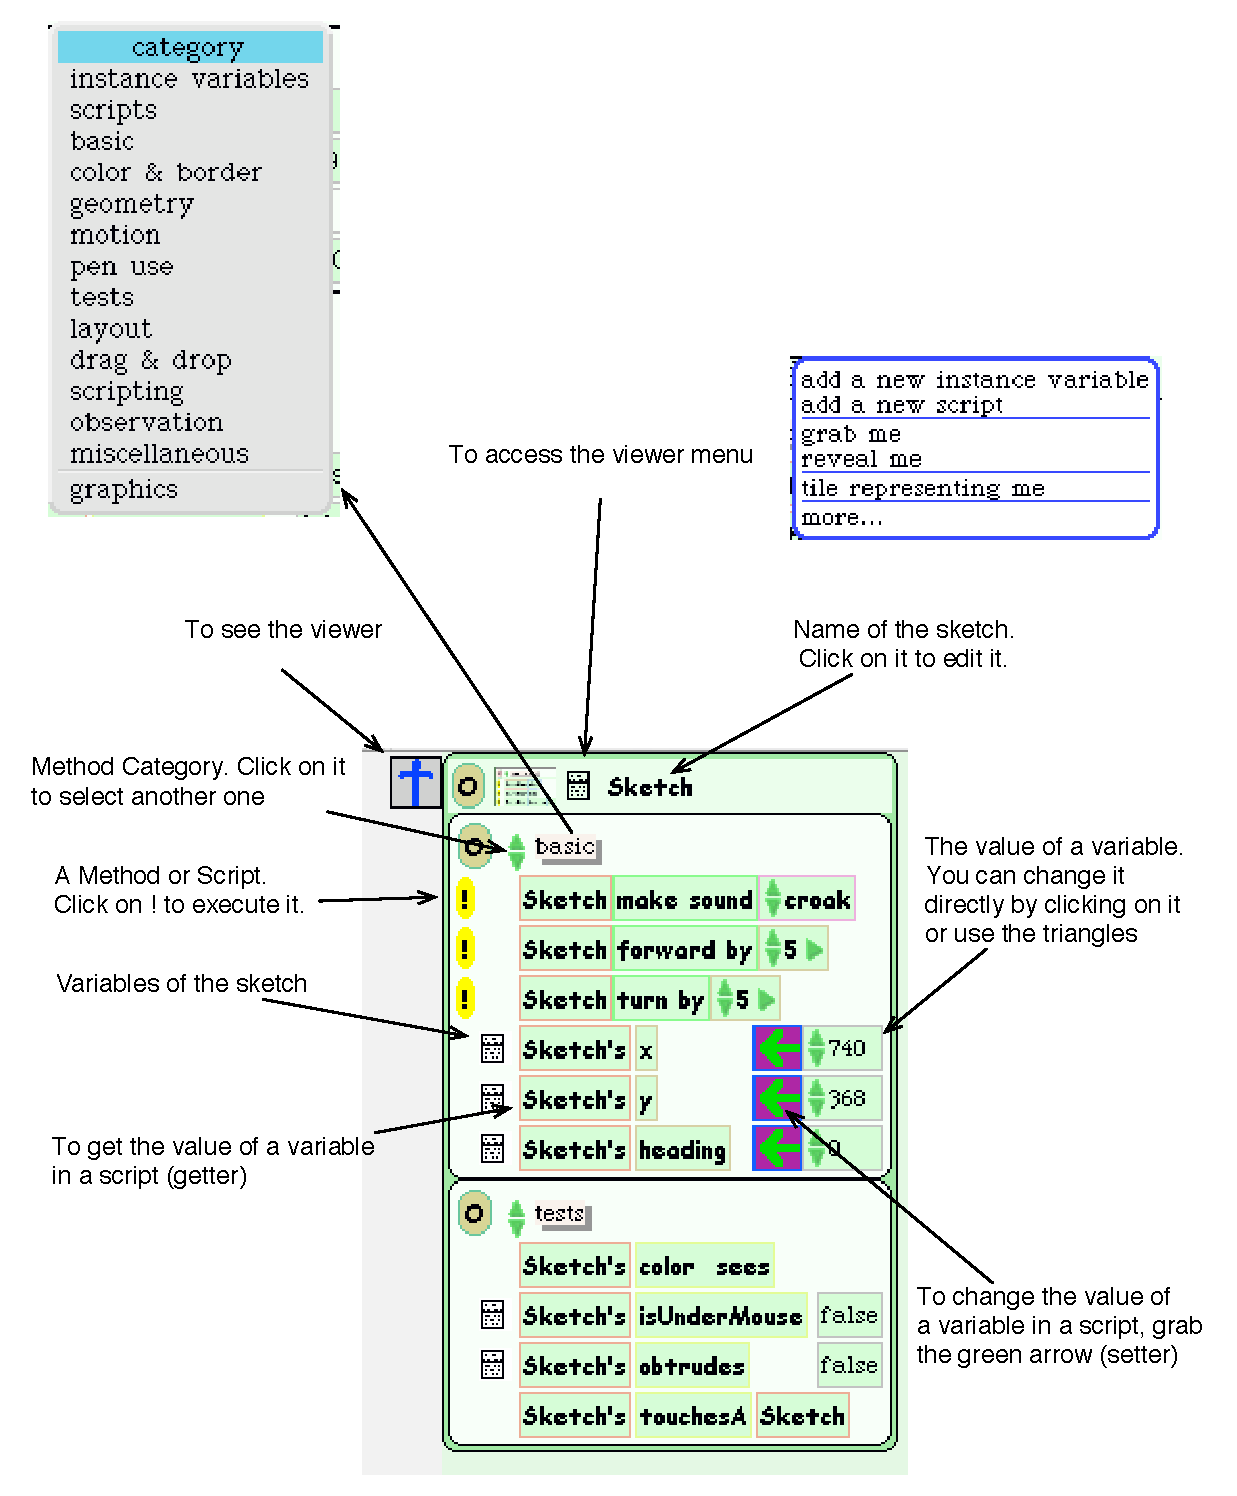
\includegraphics[width=12cm]{explainingViewer2}\end{center} \caption{Understanding a viewer.\label{fig:x}}
\end{figure}

Below each category we have the list of methods. 
When a method can be executed, there is a yellow exclamation mark in front of it. Press the exclamation mark in front of the method \ct{forward by} and you will see that the airplane is moving forward.
Then you have methods that only access variable or change variable value. We call these methods accessors: getter methods and setter methods. 

Note that you can modify directly the value of a variable by using the 
up/down green triangles or by directly typing the value in the variable box. Try for example to change the x variable to now be 800. 
In a script, as you cannot interactively change the value of a variable, you should use the getter and setter. You can get the getter for the variable x by dragging the x box in the desktop. To get the setter you should drag the big green arrow as shown by Figure~\ref{fig:x1}. 

\begin{figure}[h]
\begin{center}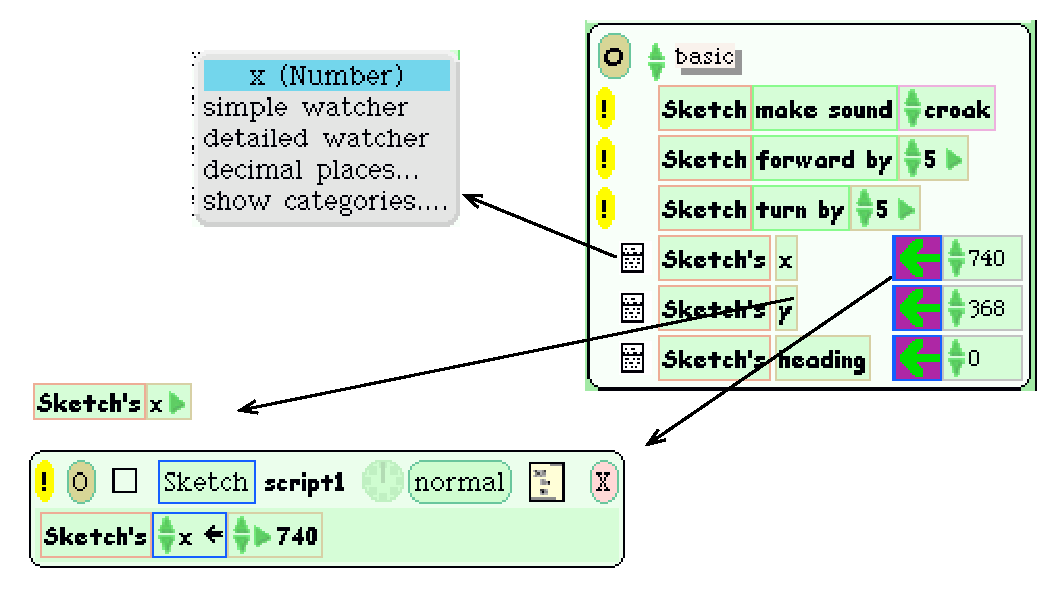
\includegraphics[width=12cm]{fromAccessorToScript} \end{center} \caption{To get access to the variables within a script. \label{fig:x1}}
\end{figure}

The number on the right of the big green arrow is the value of the variable. If you move the airplane using the brown or black halo you shall see the variables \ct{x} and \ct{y} changing their value.

You can also have watchers \ie\ ways of spying the values of variables. To create a watcher, you should click on the small menu icon that is in front of a sketch variable. You should obtain the menu displayed in Figure~\ref{fig:x2}. Then you can select to create a simple watcher which will only display the value of the variable or a detailed watcher that you can also use to change the value of the spied variable.

\begin{figure}[h]
\begin{center}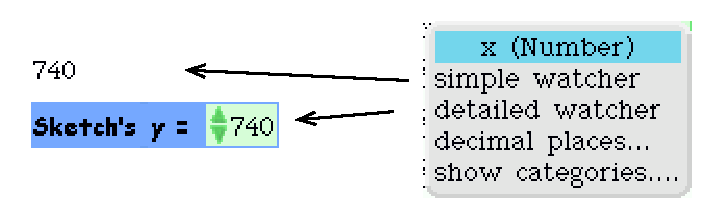
\includegraphics[width=8cm]{watchers}\end{center}
\caption{The watchers: way of spying variables. \label{fig:x2}}
\end{figure}


\paragraph{Step 3: Dragging  and Dropping a Method to Create New Scripts.}
Now if you take a method such as \ct{forward by} from the viewer and drop it on the desktop, you create a script. You should get for example the following script as shown in Figure X3. 

\begin{center}\includegraphics[width=6cm]{airplaneScr1}\end{center}
Figure X3

To execute a script you just have to click on the clock. The status of the clock is then set to ticking which means that your script is executed at regular time interval. 

\begin{center}\includegraphics[width=6cm]{script1Ticking}\end{center}

The following Figure shows the different parts of a script: there is the name of the sketch, the name of the script, a clock which lets us start and stop the script execution, the list of events the script can be linked to and the creation of conditional. 

\begin{center}\includegraphics[width=6cm]{scriptParts}\end{center}
Figure XX2


\paragraph{Step 4: Adding  Methods.} Now the airplane is getting straight when we execute the script. What we would like is that the airplane turns. To do that we should add methods into the script. Drag the method \ct{turn by} from the viewer and drop it into the script. The script should show you the place were you can drop the method by creating some green boxes. Drop the method into ones of the boxes. You should get a script that looks like the one in Figure x4. 
\begin{center}\includegraphics[width=6cm]{circle}\end{center}
Figure x 4.


Now when you execute the script, the airplane should turn in circle. In fact a sketch is similar to a turtle and you can see what the airplane is doing by asking it to put its pen down. For that look for the variable \ct{penDown} in the viewer and put its value to true as shown by the following script (see Figure X5)
.
\begin{center}\includegraphics[width=6cm]{penDown}\end{center}
Figure X5

Once the pen is down the airplane draws on the desktop as shown by Figure x6.
\begin{center}\includegraphics[]{circleDrawing}\end{center}
Figure X6

Note that you can select when the script is fired using the events button of the script. Figure X6 shows all the possible events that you can use. You can get this menu by clicking on the text right to the clock. 
\begin{center}\includegraphics[width=5cm]{events}\end{center}


%%%%%%%%%%%%%%%%%%%%%%%%%%%%%%%%%%%%%%%%%%%%%%%%%%%%
\section{Joystick in Action}
Now we would like to steer this airplane. The idea is that instead of turning always from the same amount we would like that the angle varies depending on the state of a joystick. 

\paragraph{Step 1: Creating a Joystick.}
First we create a joystick by dragging one from the supplies flaps and dropping it into the desktop. The red circle represent the top of the joystick and with it you can indicate a direction and an amount of energy put in the movement.
\begin{center}\includegraphics[]{joystickInFlaps}\end{center}

\paragraph{Step 2: Experimenting with  a Joystick.}
Second we open a viewer on the joystick using the turquoise halo. Then browsing the methods, you will find interesting methods under the category \bold{joystick}.  Move the joystick and look at the variables. The variable \ct{amount} represents the amount of energy put in the movement, \ie\ you can move the joystick in the same direction but with different strength. The variable \ct{angle} represent the direction in which you are moving the joystick and we let you guess the roles of the two other variables. 

\begin{center}\includegraphics[width=8cm]{viewerOnJoystick}\includegraphics[width=8cm]{joystickState}\end{center}

\paragraph{Step 3: Linking the Joystick and the Script.}
Now to steer the airplane we have to change the value of the method \ct{turn by} in the script
by a value given by the joystick, for example the \ct{leftRight} variable seems adequate. 
To do that drag the variable directly on the argument of the \ct{turn by} method in the script. 
It may take some times for the script to accept the variable but you should obtain the following script. 
\begin{center}\includegraphics[]{steeringFlightScript}\end{center}
Now click on the clock and steer your airplane with the joystick. As you see steering the airplane could be improved by making a difference whether we turn fast or not. Try to find a solution, the amount variable can help you for that.  

\section{Creating an Animation}

The idea for creating an animation is the following: first we draw the animations steps and put them into an animation holder. Then we create
a simple sketch whose graphical representation will be replaced by the animation elements. For this purpose we write a script that makes the sketch looking like the different steps that are contained in the holder.

\paragraph{Step 1: Holder Creation.}
To create an animation we need to create an holder. An holder is a graphical object that can contain other graphical objects. It also knows what is the currently selected item among the ones it contains. To create an holder we drag it from the red flap named supplies, and drop it into the desktop.

\begin{center}\includegraphics[]{holderInFlaps}\end{center} 
An empty holder is then created. 
\begin{center}\includegraphics[]{emptyHolder}\end{center}

\paragraph{Step 2: Drawing Animation Elements.} For the second step we draw the picture we want to animate using the paint editor presented above.  We suggest you to draw a first picture, then duplicate it using the green halo. Then select the dark grey halo to repaint the sketch. This way you can create several pictures by modifying one step by step. Here we paint a worm in two different positions. 
\begin{center}\includegraphics[width=5cm]{worms}\end{center}


Note that you can also use the red halo painting item (see Figure X7) but we suggest to use as much as possible the halos provided. 
\begin{center}\includegraphics[width=6cm]{repaint}\end{center}
Figure X7

\paragraph{Step 3: Dropping the Pictures in the Holder.}
The next step is to simply drop the resulting pictures into the holder. A black rectangle represents the currently selected picture
of the holder. 

\begin{center}\includegraphics[width=5cm]{wormInHolder}\end{center}

\paragraph{Step 4: Creating a Simple sketch Recipient of  the Animation.}
Now we need a sketch whose graphical aspect will be used as a placeholder for the animation. Therefore  we create a simple sketch for example an ellipse that we drag and drop from 
the supplies flap. Then we open a viewer on this sketch as shown by the next picture.
\begin{center}\includegraphics[width=8cm]{ellipseLookLikeA}\end{center}

\paragraph{Step 5: Creating a Script with LookLike.}
From the simple sketch, here the ellipse, we create a new script by dragging  the method \ct{lookLike dot}  (shown in he previous picture)   from the viewer to the desktop. This action should create the script described by the following picture.
\begin{center}\includegraphics[width=6cm]{scrLookLike}\end{center}

\paragraph{Step 6: Displaying the Selected Animation Element.} Now we should indicate that the ellipse should look like the
currently selected element of the holder. We select the holder and open it in a viewer as shown in the following picture. 
\begin{center}\includegraphics[width=10cm]{selectingPlayerAtCursor}\end{center}

We look for the category \ct{collection} by pressing on the basic button as shown in the following picture.
\begin{center}\includegraphics[width=6cm]{viewerCategory}\end{center}

From the list of methods we drag the method named \ct{playerAtCursor}. This method returns the player, i.e, the graphical element 
contained in the holder that is at the current position, and we drop on the square with dot in the middle (this box represents an argument of the method lookLike). We obtain the following script. 
\begin{center}\includegraphics[]{scr2Ani2}\end{center}

\paragraph{Step 7: Changing the Currently Selected Element of a Holder.}
If we execute the previous script using the ticking button, the script will just change the shape of the 
ellipse to be the currently selected graphical element. We do not have an animation yet. For that we need to find a way to change
the currently selected item of an holder. In fact, an holder has an index, named cursor,  that represents the rank of the currently selected item. It suffices to increment such an index to make the holder selecting another graphical element. 

To change the value of the variable named \ct{cursor}, we drag the arrow (shown on the right in the next figure), on the following line of the previous script. 
\begin{center}\includegraphics[]{mutator}\end{center}
We obtain the next script which say the the variable contains the value 1. 

\begin{center}\includegraphics[]{scr2Ani3}\end{center}

Now if you click on the double green triangles of the setter in the script you will see that there is the possibility to increase the cursor by a given amount as shown in the following script. 
\begin{center}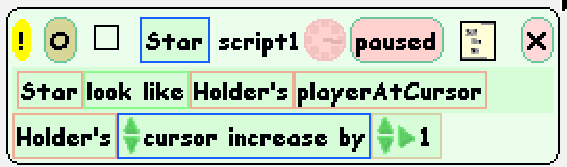
\includegraphics[]{scr2Ani3bis}\end{center}

Now your animation should work. 

\paragraph{Another Way.}
To achieve the same effect we can also reproduce the expression \ct{cursor := cursor +1} that will move the cursor to the next element. Therefore we drag the left part of the cursor from the viewer at the place of the 1 in the script and we get the following script. 
\begin{center}\includegraphics[width=6cm]{scr2Ani4}\includegraphics[width=6cm]{scr2Ani5}\end{center}
Now we just have to click on the small green triangle at the end of the cursor box in the script to make appear a plus 1 expression 
as shown in this final script. As you see the first solution is easier.

We suggest the reader interested to use eToy in his classroom to read the eToy book we mentioned in the start of this chapter, as it presents a lot of pedagogical aspects that can be used with this example. 


%%%%%%%%%%%%%%%%%%%%%%
\section{Cars and  Drivers}

Now we would like to show you how we can build a script to drive a car with a wheel. This exercise is used for teachers to show the use of division to act as a demultiplior as in real cars, but this is also fun to do.

\paragraph{Step 1: Draw a Car and a Wheel.} Using the painter editor draw a car and a wheel. 

\begin{center}\includegraphics[width=4cm]{car}\hspace{1cm}\includegraphics[]{wheel}\end{center}

\paragraph{Step 2: Car Turning in Circle.} Open a viewer on the car, rename the sketch to be named 'car',  then drag and drop
the method \ct{forward} as we previously did. The following script  should be created.
\begin{center}\includegraphics[]{carForward}\end{center}
Then drag and drop the method \ct{turn} below the previous method in the newly created script. You should obtain the 
following script that when run makes the car going in circle. 
\begin{center}\includegraphics[]{carForwardTurn}\end{center}

\paragraph{Step 3: Use Wheel Heading.}
Now we should link the angle of which the car turns with the wheel. We should find a way to rotate the wheel and know the amount of rotation. The first problem is easy to solve: If you bring the halos, click on the blue halo and turn. This rotates the wheel.
Now for the second problem, open a viewer on the wheel, rename it wheel,  look for the \ct{heading} variable in the viewer  (the expression should be \ct{wheel's heading}). When you rotate the wheel using the halo, the value of the variable changes. This variable represents the rotation angle compared to the original picture.

\begin{center}\includegraphics[]{wheelHalos}\end{center}

Now we have all the pieces of the puzzle, we have to indicate that the car should turn not from a fix amount but
from the wheel's heading. To do that drag the expression \ct{wheel's heading} from the viewer onto the number 5 argument of the 
\ct{turn} method in the previous script. You should have now the following script. 
\begin{center}\includegraphics[]{carSteering}\end{center}

Now if you click on the small clock of the script, it runs and using the blue halo of the wheel you can control 
the car. However as you will notice this is not really perfect. Normally kids should emit hypothesis about the problem and try solution.

The problem is that we should divide the wheel's heading value to get a finer control when we are turning. To do that click on the rightmost small green triangle of the wheel's heading block. This adds extra boxes. Click on them to select the division \ct{//}. You have now a script that looks like the following one.
\begin{center}\includegraphics[]{carGoodSteering}\end{center}

Have fun controlling your car. 
\begin{center}\includegraphics[]{carWheel}\end{center}


%%%%%%%%%%%%%%%%%%%%%%%%%%%%%%%%%%%%%%%%%%%%%%
\section{Automatic Cars}
Now we would like to program the car so that it finds its way on a road automatically. The idea is to equip the car with some sensors
that tell it whether it is going off the road. Once the car is equipped with sensors and we program it, we want to put the car on the road and it should follow the road. 

Note that here we will not show you a working solution because we believe that this is much better for you to experiment. Our solution in fact does not really work. 

\paragraph{Step 1: Sensors.}
In eToy we can ask whether a certain color of a sketch sees another color under it. We can use this capability to have sensor. A sensor will then be a simple dot of color that will tell the car if it is passing above another color. To equip our car with sensors, we repaint the car and add two dots of colors as shown by the following figure. 
\begin{center}\includegraphics[]{carWithSensor}\end{center}

\paragraph{Step 2: The Road.} Using the paint editor now we create a road with one single color. We suggest you to try later  with different bands of colors to see how you have to change the behavior of the car.

\begin{center}\includegraphics[]{road}\end{center}

\paragraph{Step 3: Condition and Tests in Etoy.}
Open a viewer on the car then drag and drop the method \ct{forward by} into the desktop. This creates a script that you normally get used. 

Now we need to have a way to express different behavior depending on the sensor value. For that purpose we need to have the possibility to express a condition or a test. To get test you should drag the second from the right small pale square box at the top of the script near the cross button (see Figure XX2). So drag and drop such a tile test in the script, you should now get a script which looks 
like the following one.
\begin{center}\includegraphics[]{carForwardTestEmpty}\end{center}

Now we need to find a way to make our sensors active. Look and find the method \ct{color sees} in the category \ct{test} as shown below. This method returns true or false depending whether a colored part of the sketch of a given color passes over another color. 
\begin{center}\includegraphics[width=6cm]{carTestProcotol}\end{center} 

Drag such a method into the script besides the word Test. You should obtain a script similar to the following one. 
\begin{center}\includegraphics[]{carTestBasic}\end{center}

\paragraph{Step 4: Customizing Color-based Tests.}
Now we should have a way to define the color that the test should use. This is easy, we have to click on the colored square that is inside the method \ct{color sees} itself. This automatically opens a color picker (see Figure YX). With the color picker picks the color  
of one sensor. The first color of the script should chane to reflect the color you selected. Do the same operation for the second colored box but this time pick the color of the road.  
\begin{center}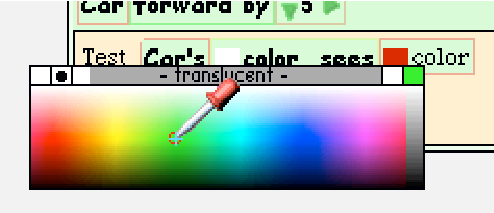
\includegraphics[]{colorPicker}\end{center}
Figure YX
\begin{center}\includegraphics[]{carTestNotFinished}\end{center}

\paragraph{Step 5: Adding Actions.}
Now we can specify that the car should turn when the sensor does not see the color of the road. We just have to drag and drop the method \ct{turn by} besides the word No in the script. Now you can pick the car, put it on the road and press the clock to run the script. 
\begin{center}\includegraphics[]{carFollowingRoad}\end{center}

Obviously the behavior is not perfect and we let you change it or define your own solution. 



\section{Some Tricks}
We just want to show you some aspects that may help you. The eToy environment can be customized, we suggest you to open the menu \menu{playfield options...} and let your mouse wander on the different items and read the balloon help.

\begin{center}\includegraphics[]{playfieldOptionMenu}\end{center}

\paragraph{Running Several Scripts.} If you create several scripts they will run in parallel. To control all the scripts available on the desktop you can use the widget named All Scripts that is available in the \menu{widget} flaps. Once you drop this widget in the desktop you get a panel that allow you to run and stop all the scripts currently on the desktop. 

\begin{center}\includegraphics{scriptRunner}\end{center}

Note that you can also use the method \ct{start script} and the related method contained in the category \ct{scripting} to start, pause, or stop scripts.

\begin{center}\includegraphics[width=6cm]{startScript}\end{center}
It is interesting to see that one script can invokes the exuction of other scripts. This let you create more complex scripts. 

\paragraph{Cleaning.} You can clean all the turtle trails using the method \ct{clear all pen trails} that is available in the category \ct{pen use}.

You can also clean the desktop from the traces \index{clear the trails} made by the players. For that purpose use the last menu item of the menu \index{appearance menu} \menu{appearance} that you can get from the \menu{World} menu. 

\paragraph{Making A Tile.}
if you want to write a script which links two objects, you sometimes need to refer to this object. In such a case,you need to have a tile that represents the object to drop it in your script. Let us take an example, imagine we have two airplanes one blue and one red and we want the red to follow the blue one. We use then the method \ct{move toward} as shown below. 

\begin{center}\includegraphics[]{moveToward}\end{center}
Now as we want that the red airplane move toward the blue airplane and not the dot as in the previosu script. We first use the orange halo of the blue airplane to get a tile representing it.
\begin{center}\includegraphics[]{makeAtile}\end{center}
Then we drop this tile in the script. Now the red airplane is fllowing the blue one.
\begin{center}\includegraphics[]{following}\end{center}


\paragraph{Internationalization.} Now if you want to use eToy with small kids, you can choose the language you want. Sometimes the complete \sq interface is translated. Bring the World menu, select the item \menu{help...} followed by \menu{the set language...}.

\begin{center}\includegraphics[width=6cm]{language}\end{center}
\begin{center}\includegraphics[width=10cm]{spanishEtoy}\end{center}

%\section{A Final Remark}
%You may wonder why we did not write a book on eToy and why we chose to build our own  environment. There are several reasons that explain our choice. First eToy was and is still a work on progress developed by the team of Alan Kay. It was difficult for us to know all the details of the system and to understand all the possibilities and limits. This is after seeing demoes made by the \sq team that we understood the possibilities offered. Now a book is available but in 1998 when we started nothing was available. Second, my wife was in a difficult situation because she was starting to teach computer science for the first time and she had to prove that she was good, especially to the students because the previous teacher was just fired. Therefore we could not do any experimentation, an hesitation would have been perceived as an error. 

%With the turtle environment we controlled completely the system which started with two simple classes, and I wrote a first version of this book in french with precise exercises and goals. Third, my initial goal is to teach programming and in the particular context object-oriented programming. Another book focusing on object-oriented programming is following. The model underneath the eToy system is based on events (ticking) and more concurrent-like model of computation. Loops for example are not explicit but omnipresent because the events are triggered on regular time basis. For all the reasons I decided to write my own material. 


Again this is just a survey of the possibilities of Etoy and I suggest you to go to \ct{http://www.squeakland.org} and check the material available there. 
\ifx\wholebook\relax\else
\end{document}\fi
